\documentclass[compress]{beamer}
\usepackage{ifthen,verbatim}

\title{Update on alignment and studies of residual misalignment on TeV dimuons}
\author{Jim Pivarski, Alexei Safonov}
\institute{Texas A\&M University}
\date{15 May, 2008}

\newcommand{\isnote}{}
\xdefinecolor{lightyellow}{rgb}{1.,1.,0.25}
\xdefinecolor{darkblue}{rgb}{0.1,0.1,0.7}

%% Uncomment this to get annotations
%% \def\notes{\addtocounter{page}{-1}
%%            \renewcommand{\isnote}{*}
%% 	   \beamertemplateshadingbackground{lightyellow}{white}
%%            \begin{frame}
%%            \frametitle{Notes for the previous page (page \insertpagenumber)}
%%            \itemize}
%% \def\endnotes{\enditemize
%% 	      \end{frame}
%%               \beamertemplateshadingbackground{white}{white}
%%               \renewcommand{\isnote}{}}

%% Uncomment this to not get annotations
\def\notes{\comment}
\def\endnotes{\endcomment}

\setbeamertemplate{navigation symbols}{}
\setbeamertemplate{headline}{\mbox{ } \hfill
\begin{minipage}{5.5 cm}
\vspace{-0.75 cm} \small
\end{minipage} \hfill
\begin{minipage}{4.5 cm}
\vspace{-0.75 cm} \small
\begin{flushright}
\ifthenelse{\equal{\insertpagenumber}{1}}{}{Jim Pivarski \hspace{0.2 cm} \insertpagenumber\isnote/\pageref{numpages}}
\end{flushright}
\end{minipage}\mbox{\hspace{0.2 cm}}\includegraphics[height=1 cm]{../cmslogo} \hspace{0.1 cm} \includegraphics[height=1 cm]{../tamulogo} \hspace{0.01 cm} \vspace{-1.05 cm}}

\begin{document}
\frame{\titlepage}

%% \begin{notes}
%% \item This is the annotated version of my talk.
%% \item If you want the version that I am presenting, download the one
%% labeled ``slides'' on Indico (or just ignore these yellow pages).
%% \item The annotated version is provided for extra detail and a written
%% record of comments that I intend to make orally.
%% \item Yellow notes refer to the content on the {\it previous} page.
%% \item All other slides are identical for the two versions.
%% \end{notes}

\begin{frame}
\frametitle{Outline}
\begin{itemize}\setlength{\itemsep}{0.75 cm}
\item Status of alignment algorithms in iCSA08
\item Plans for studying residual misalignments on TeV muons
\item $Z'$ MC samples and Zprime2muAnalysis in 2\_0\_X
\end{itemize}
%% \hspace{-0.83 cm} \textcolor{darkblue}{\Large Outline2}
\end{frame}

\begin{frame}
\frametitle{Status of alignment}

HIP-based muon alignment has matured

\vspace{0.25 cm}
\begin{itemize}\setlength{\itemsep}{0.25 cm}
\item same basic idea: extrapolate tracker-fitted tracks into the muon
system, align chambers to these tracks
\begin{itemize}
\item simultaneously aligns muon system internally and muon system to tracker
\end{itemize}
\item major correction from CSA07 experience (direction of refit)
\item numerous bug-fixes and minor corrections improved resolution
\item now in few-hundred micron range for inner stations
\item separate ``baseline'' procedure from commissioning procedures
that operate without tracker or magnetic field (e.g. CSC overlaps
technique and related layer-alignment technique)
\end{itemize}

\end{frame}

\begin{frame}
\frametitle{iCSA08 tests}

All tracker and muon alignment algorithms are being tested in
1~pb$^{-1}$ (this week) and 10~pb$^{-1}$ (next week) challenges

\vspace{0.25 cm}
\begin{itemize}
\item full-spectrum event samples, including muons from QCD
\item original track fits were misaligned (important!)
\item up-to-date initial misalignment scenarios
\item tracker alignment and muon HIP alignment performed in series
\end{itemize}

but\ldots
\begin{itemize}
\item samples correspond to unequal integrated luminosities
\item no layer misalignments in muon system
\end{itemize}

\vfill
Martin Weber (tracker alignment) and I decided to do a more realistic
study after timed CSA test is over

\end{frame}

\begin{frame}
\frametitle{Results from pre-CSA test}

Pre-CSA test approximates upcoming CSA 10~pb$^{-1}$ results

Chamber $r\phi$ positions before (gray) and after (yellow) alignment

\begin{center}

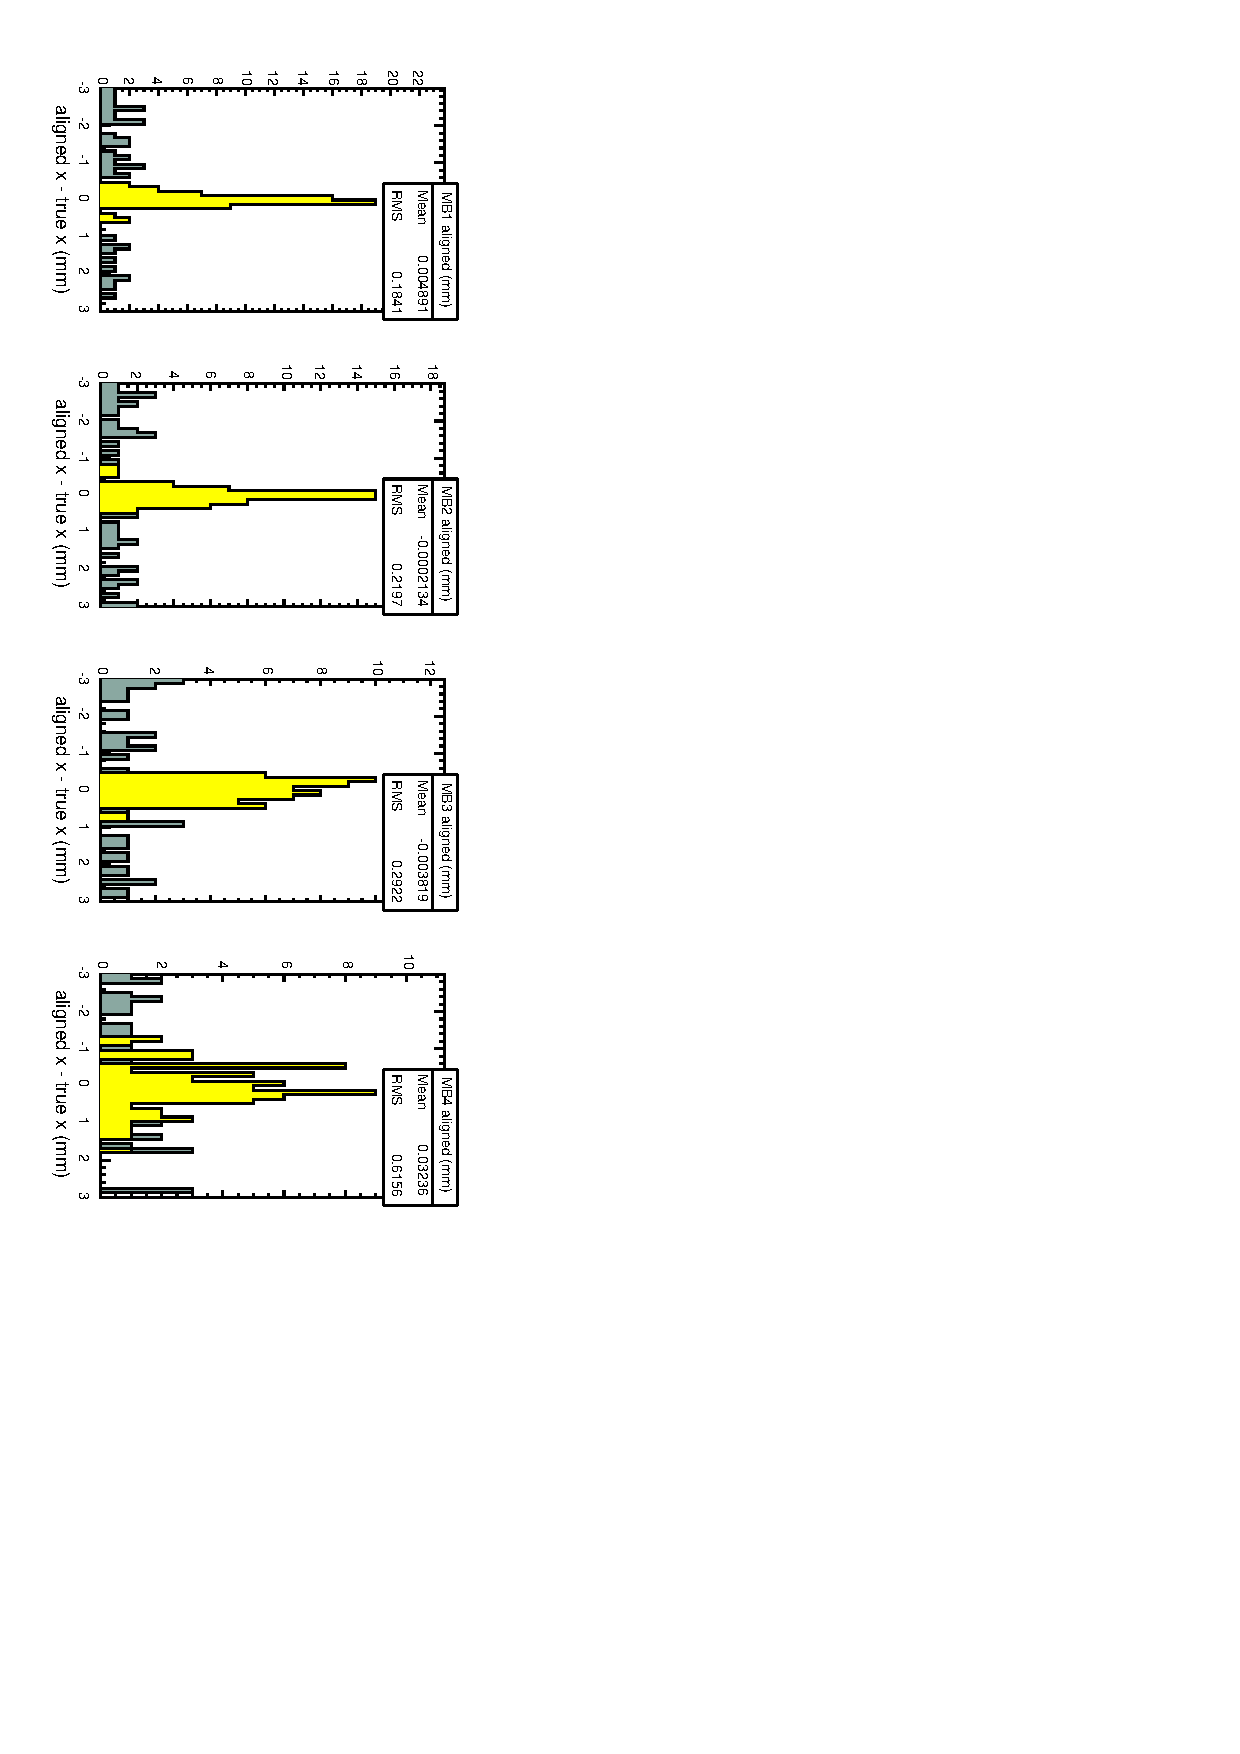
\includegraphics[height=0.85\linewidth, angle=90]{barrel_184.pdf}

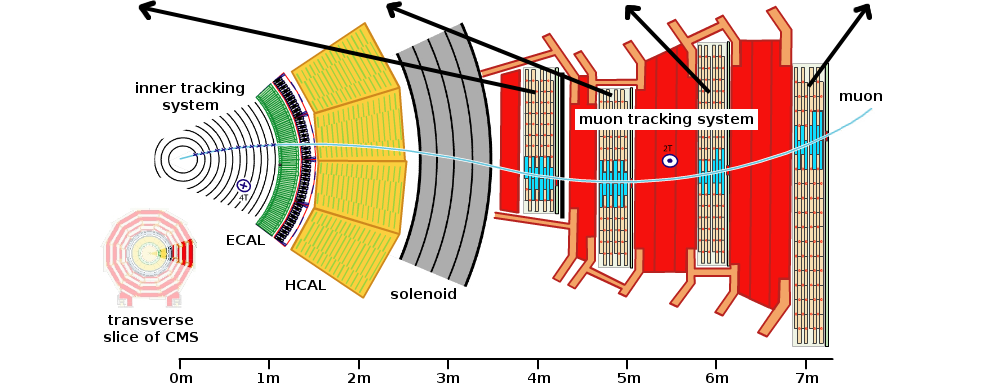
\includegraphics[width=0.85\linewidth]{cms_slice.png}

\end{center}

\end{frame}

\begin{frame}
\frametitle{Effect of misalignment on tracks}

\begin{itemize}\setlength{\itemsep}{0.5 cm}
\item Tracker and muon alignment output from post-CSA study will be a
good starting point for quantifying the effects of misalignment on
tracks, specifically TeV muons

\item Alignment is in 2\_0\_6, misalignment study would be in 2\_0\_X,
suitable for Muon POG note (twiki MuonPOGRecoNote)

\item Would also come at the right time for Piotr's TeV reconstruction
study

\item Ivan and I have roughly split misalignment studies into basic
resolution plots (me), shift of peak (me?), charge mismeasurement, effect
on efficiency (Ivan)

\end{itemize}

\end{frame}

\begin{frame}
\frametitle{MC samples/Zprime2muAnalysis}

New $Z'$ samples in

{\tt /castor/cern.ch/user/p/pivarski/Zprime\_206\_FEVTSIM/}

\begin{itemize}
\item New CMSSW version: we can do MPOG tests, use latest alignment
\item Enough saved for track re-reconstruction and Zprime2muAnalysis
\item Same generator-level cuts as CSA07 samples
\item 1500 1~TeV, 1500 2~TeV, 1000 3~TeV
\item Can be viewed as provisional if new official $Z'$ samples are coming
\end{itemize}

\vfill
Zprime2muAnalysis
\begin{itemize}
\item I plan to do all resolution studies in Zprime2muResolution
\item Jordan is bringing the package up-to-date (compiles in 2\_0\_6)
\end{itemize}

\end{frame}


%% \section*{First section}
%% \begin{frame}
%% \begin{center}
%% \Huge \textcolor{blue}{First section}
%% \end{center}
%% \end{frame}

\begin{frame}
\frametitle{Summary}

\begin{itemize}\setlength{\itemsep}{0.5 cm}
\item A lot of progress on alignment algorithms
\item iCSA08 is underway, will provide reliable predictions of misalignment at 1 and 10~pb$^{-1}$
\item Preparing tools for studying misalignment
\end{itemize}

\label{numpages}
\end{frame}

\end{document}
